%%
%%                  TEMPLATE for Math 436 project report
%%
\documentclass[11pt]{amsart}
%%% WARNING: Do NOT change the page size, fonts, or margins!  Penalties will apply.


\usepackage{graphicx}
\usepackage{amssymb,amsmath,amsthm}
\usepackage{placeins} %enables \FloatBarrier, which prevents figures and tables from going below it.
\usepackage{hyperref} %makes cross references into hyperlinks. 
 

%%% WARNING: Do NOT change the page size, fonts, or margins!  Penalties will apply.
%%% WARNING: Do NOT change the page size, fonts, or margins!  Penalties will apply.

\begin{document}

\title{Modeling Salvation}
\author{Taylor Rubalcava, Matthew Ward, Matthew  Dangerfield}

% Change the date to match the date you actually wrote this paper
\date{\today} % or use \today

\begin{abstract}
Using key indicator data generated by The Church of Jesus Christ of Latter-Day Saints' missionaries, this paper studies the potential for modeling the growth of church membership in local regions using a simple modification of the SIR model. This model exhibits many of the qualitative behaviors experienced by missionaries on a local scale and is capable of giving reasonable estimates for church membership growth in a local region over the short term. Using this simple model, the potential impacts of changes in the missionary program can be studied and opportunities for potential growth can be found.
\end{abstract}

\maketitle % this actually makes the title

%% First Section
\section{Background/Motivation}

The Church of Jesus Christ of Latter-Day Saints has approximately 70,000 missionaries serving in voluntary ecclesiastical service around the world \cite{Church1}. To organize this massive coalition of young adults (usually 18-23 years old) in foreign countries, the church has a series of 'Key Indicators' that can effectively be thought of as steps in a conversion funnel.

\begin{itemize}
  \item New People (number of individuals beginning to be taught by missionaries)
  \item Sacrament Attendances (number of individuals attending worship services)
  \item People on Date (number of individuals who have scheduled a day to join the church)
  \item Baptisms (number of individuals who have joined the church via baptism)
\end{itemize} \cite{Church2}

These key indicators are used as a metric of success by the missionary department, the missionaries themselves, and represent the experiences of thousands of missionaries and the hundreds of thousands that they teach. A model of the key indicators could be used to explore the impacts of policy change and predict the effects of various situations on church membership. 

A person's contribution to these key indicators represents their progression towards become a member of The Church of Jesus Christ of Latter-Day Saints.

A mathematical model that can simulate the impacts of these leadership decisions, prior to their enactment, would be invaluable in avoiding pitfalls and analyzing opportunities for growth. Indeed, the conversion funnel that the missionaries' key indicators represent is similar to those of other organizations including sales funnels, a population's conversion to a particular political or other philosophy, and (similar to both the benevolent and malevolent memetic means present in each of these examples) actual viruses.

For this reason a modified version of the prototypical SIR model was used. Unlike the SIR model, however, the model developed here allows for individuals to progress forwards and backwards through the various key indicators. We believe that this is a more realistic model not only for the missionaries but also various other phenomena such as the ones mentioned above. Ultimately our goal is two-fold, to model missionary key indicators, and thus church membership, over time. 

We are unaware of any previous efforts to model the missionaries' key indicators.

%% Second Section 
\section{Modeling}

\begin{center}
    \textbf{Simplifying assumptions.}
\end{center}

In order to model this complicated system with ODEs, we make the following simplifying assumptions.

\begin{itemize}
    \item All people fall into one of the following ordered categories:
    \begin{enumerate}
        \item Uncontacted
        \item Being taught
        \item Attending Church meetings
        \item On date to join the Church
        \item Church members
    \end{enumerate}
    \item In their progression and regression, people do not skip categories. For example, a person who is uncontacted (1) cannot immediately begin attending Church meetings (3), or vice versa.
    \item Unless otherwise stated below, the rate at which people progress or regress in any category is proportional to the number of people in that category.
    \item Since missionaries have by far the most success when Church members refer their friends for missionary discussions, the rate at which uncontacted people (1) start being taught (2) is also proportional to the number of members of the Church.
    \item We choose not to model those who choose to withdraw from Church membership, so the rate of regression from membership (5) is zero.
\end{itemize}

\vspace{1em}
\begin{center}
    \textbf{Constructing the model.}
\end{center}
\nopagebreak

Let $p_i$ with $i \in \{1, ..., 5\}$ represent the proportions of the population that are uncontacted ($p_1$), being taught ($p_2$), attending sacrament meeting ($p_3$), on date to be baptized ($p_4$), and Church members ($p_5$). These are each functions of time. Together they compose the vector function $\boldsymbol{p}(t) = \left(p_1(t), ..., p_5(t)\right)$.

Each $p_i$ has two rates $\alpha_i(t)$ and $\beta_i(t)$ (these may also depend on time) attached to it. $\alpha_i$ is the rate they progress towards joining the Church ($p_i \rightarrow p_{i+1}$), and $\beta_i$ is the rate they regress away from joining the Church ($p_i \rightarrow p_{i-1}$). Hence, setting $p_0$ and $p_6$ (as well as their respective rates $\alpha_0$, $\beta_0$, $\alpha_6$, and $\beta_6$) equal to 0 for ease of notation, letting $t$ represent time, and using Newton's dot-notation for derivatives, for all $i \in \{1, ..., 5\}$ it holds that:

\begin{equation}
\dot{p}_i(t) = \alpha_{i-1}(t) p_{i-1}(t) + \beta_{i+1}(t) p_{i+1}(t) - (\alpha_i(t) + \beta_i(t)) p_i(t)
\label{eq:OrigModel}
\end{equation}

We set $\alpha_5(t) = 0$ since we assume no progression beyond joining the church, we set $\beta_1(t) = 0$ since we assume no regression beyond being uncontacted, and we also set $\beta_5(t) = 0$, since we assume that once a person has joined the church, they do not leave it.

In Equation~\ref{eq:OrigModel}, at the stage of progression $p_i$, $\alpha_{i-1} p_{i-1}$ is the rate at which people progress from the lower stage into stage $p_i$, and $\beta_{i+1} p_{i+1}$ is the rate people regress back to $p_i$ from the next stage along.

The rate at which uncontacted people start being taught is proportional to the number of members, so $\alpha_1(t) = a_1 p_5(t)$ for some constant $a_1$. In this sense, $a_1$ may be thought of as the number of new people being taught per member per unit time. So fix constants $\{a_1, ..., a_4\}$ and $\{b_2, ..., b_4\}$ and define

\begin{equation}
\begin{aligned}
    \alpha_i(t) &= \begin{cases} 
    a_1 p_5(t) & \text{if } i = 1, \\
    a_i & \text{if } i \in \{2, ..., 4\}, \\
    0 & \text{otherwise}
    \end{cases} \\
    \beta_i(t) &= \begin{cases} 
    b_i & \text{if } i \in \{2, ..., 4\}, \\
    0 & \text{otherwise}.
    \end{cases}
\end{aligned}
\label{eq:Rates}
\end{equation}


for all times $t$.

This model is a slight adaptation of the prototypical SIR model, which only allows for forward movement or progression of individuals through states. This model not only allows for backwards movement but it allows for it at every state. 

In summary, combining Equations ~\ref{eq:OrigModel} and ~\ref{eq:Rates}, representing each $p_i(t)$ simply as $p_i$, and representing element-wise multiplication by $\circ$, we have that

\begin{equation}
    \boldsymbol{\dot{p}}
        =
    \begin{pmatrix} \dot{p_1} \\ \dot{p_2} \\ \dot{p_3} \\ \dot{p_4} \\ \dot{p_5} \end{pmatrix}
        =
    \begin{pmatrix} 0 \\ a_1 p_5 \\ a_2 \\ a_3 \\ a_4 \end{pmatrix} 
        \circ 
    \begin{pmatrix} 0 \\ p_1 \\ p_2 \\ p_3 \\ p_4 \end{pmatrix} 
        + 
    \begin{pmatrix} b_2 \\ b_3 \\ b_4 \\ b_5 \\ 0 \end{pmatrix} 
        \circ 
    \begin{pmatrix} p_2 \\ p_3 \\ p_4 \\ p_5 \\ 0 \end{pmatrix} 
        - 
    \left(\begin{pmatrix} a_1 p_5 \\ a_2 \\ a_3 \\ a_4 \\ 0 \end{pmatrix} + \begin{pmatrix} 0 \\ b_2 \\ b_3 \\ b_4 \\ 0 \end{pmatrix}\right) 
        \circ 
    \begin{pmatrix} p_1 \\ p_2 \\ p_3 \\ p_4 \\ p_5 \end{pmatrix}
\label{eq:VectorizedModel}
\end{equation}

\vspace{1em}
\begin{center}
    \textbf{Setting parameters.}
\end{center}

\nopagebreak

To show that our model has the behavior we expect, we set the parameters and initial conditions in a reasonable way and observe the results. We let the unit of time be weeks, beginning at $t=0$ so that $\boldsymbol{p}(3)$ represents the state of the system at 3 weeks.

\textit{Initial conditions:}
\begin{itemize}
    \item $p_1 = 0.999$. The vast majority of the population is uncontacted.
    \item $p_2, p_3, p_4 = 0$. Nobody is being taught, attending sacrament meeting, or planning to join the Church.
    \item $p_5 = 0.001$. Church members represent a small proportion of the population.
\end{itemize}

\textit{Parameters:}
\begin{itemize}
    \item $a_1 = \frac{1}{100}$. 1 person begins receiving discussions per 100 Church members per week.
    \item $(a_2, a_3, a_4) = (\frac{1}{3}, \frac{1}{20}, \frac{1}{12})$. Other progress rates (people per week).
    \item $(b_2, b_3, b_4) = (\frac{1}{15}, \frac{1}{2}, \frac{1}{2})$. Rates of regression (people per week).
\end{itemize}

\vspace{1em}
\begin{center}
    \textbf{Long-term simulation.}
\end{center}

\nopagebreak

Using the initial conditions and parameters given above, we begin by simulating a long period of time---500 years (see Figure ~\ref{fig:LongTerm}). We see that as Church membership grows, missionary work accelerates, as our assumptions would imply. Subsequently, as Church memberships approaches 100\%, missionary work slows. 

\begin{figure}[htb]
\begin{center} %Put your images in a figure like this
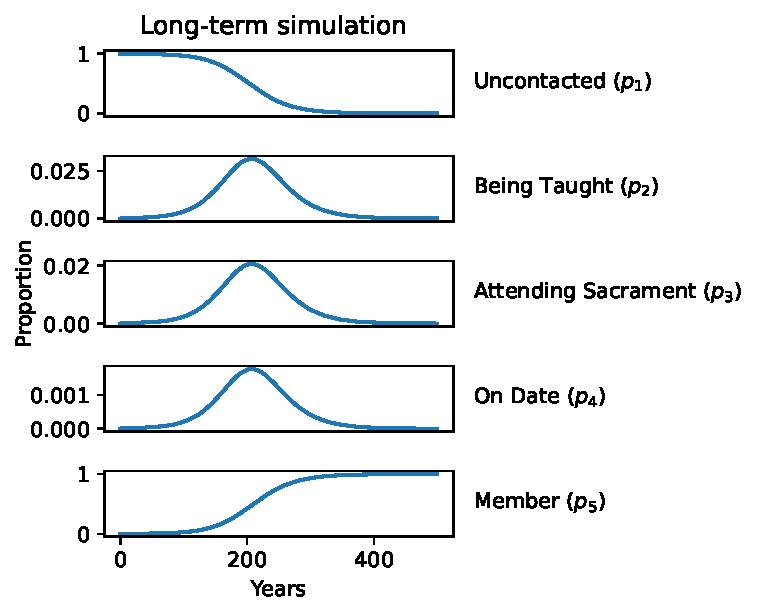
\includegraphics[width=0.85\textwidth]{long-term.pdf}
\end{center}
\caption{500 years of missionary work simulated with plausible initial conditions and parameters. Around 200 years, the rate of increase in membership is maximized.}
\label{fig:LongTerm}
\end{figure}



\begin{figure}[htb]
\begin{center} %Put your images in a figure like this
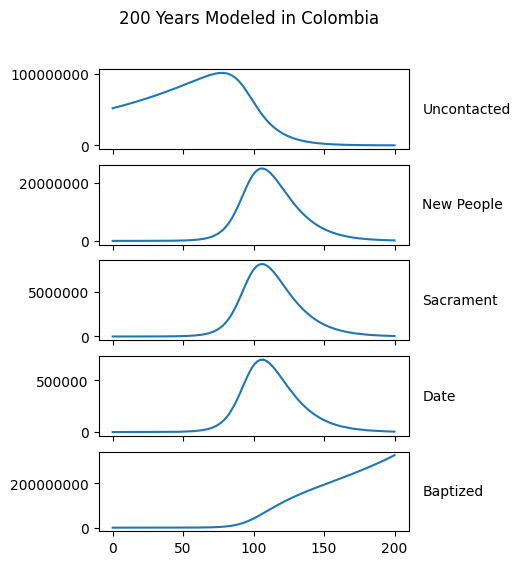
\includegraphics[width=0.75\textwidth]{200YearsColombia.png} % Better to make them pdfs than png or gif or jpeg
\end{center}
\caption{Predicting 150 years into the future how church membership will grow in Colombia.}
\label{fig:Colombia200} % for automatic cross referencing
\end{figure}

%When trying to fit the model to real world short-term data, however, we see that the model struggles to capture certain trends, especially among the $n$ (new) category of people (see Figure~\ref{fig:FitColombia}. While the $b$ (baptized people) category is accurately captured, the wild increase and decrease of $n$ (new people) in the real data is not.

\begin{figure}[htb]
\begin{center} %Put your images in a figure like this
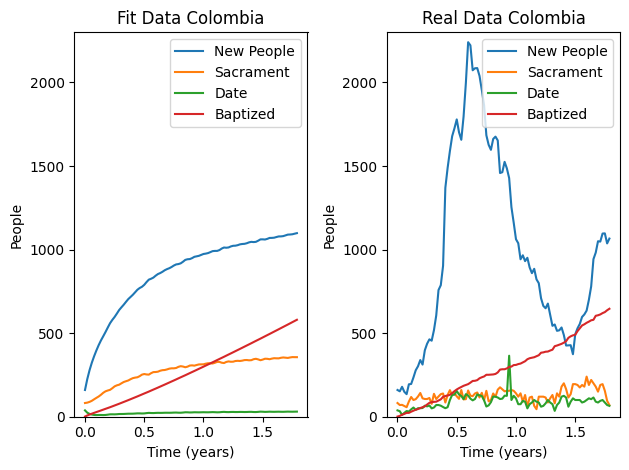
\includegraphics[width=1\textwidth]{FitColombia.png} % Better to make them pdfs than png or gif or jpeg
\end{center}
\caption{Fitting our model to real data from the Colombia Cali mission between 2021 and 2023. While the $b$ (baptized people) category is accurately captured, the wild increase and decrease of $n$ (new people) is not. This is to be expected given that the rates in our model are fixed over time.}
\label{fig:FitColombia} % for automatic cross referencing
\end{figure}


%% Third Section
\section{Results}

The model does display many of the quantitative and qualitative behaviors that would be expected from the key indicators. This includes the transient populations (new people, people attending sacrament, and people on date) remaining fairly constant in the short term, reasonable proportions between the various person states, and projecting approximately the same number of individuals being baptized as there actually were. Interestingly the model also displays some of the same oscillatory behaviors observed in the real key indicators, but doesn't seem to find a strong relationship between the transient person states and the number of individuals that will be baptized. Long term estimates are incredibly sensitive to the initial parameters, however, suggesting that the future growth of the church is highly sensitive to the world's population growth, the population growth of the church itself, and numerous other factors that are not accounted for in this model.

When used to model real mission data, as in Figure~\ref{fig:FitColombia}, we see that because the parameters are fixed, the model cannot capture the unpredictability of real-life missionary work in the short term. It can, however, model longer-term trends.

We concluded that the model could be useful while exploring the potential impacts of policy changes in the short term but is unstable and unlikely to be helpful while making long-term predictions. 

%%Fourth Section
\section{Analysis/Conclusions}

We believe that the adapted SIR model presented here is a reasonable choice for modeling church population in the short term (i.e. less than 50 years) but perhaps an unreasonable choice for modeling missionary key indicators. Generally, we failed to accurately model the real world key indicator data that is available to us, particularly 'New People'. The data does not exhibit some of the behavior necessary for the assumptions that the SIR model is based on, namely that individuals move from one key indicator to the next at a rate proportional to their respective populations. The key indicators (specifically new people) do not generally exhibit this behavior, namely with the population of those attending sacrament not increasing at a rate proportional to the population of new people.

We did, however, model church membership in a local area fairly accurately. Just as with virus modeling, and thus from an SIR perspective, this makes sense as we would expect a proselytizing church population to grow at a rate proportional to the number of members. Given the accuracy of the model while predicting church membership, and the original SIR model's ability to predict the evolution of a system, this or a similar model may be capable of predicting the plateau of church membership.


%%%%%%%%%%%%%%%%%%%%%%%%%%%%%%%%%%%%%
%% Bibliography below
%%%%%%%%%%%%%%%%%%%%%%%%%%%%%%%%%%%%%
\FloatBarrier % Keep the figures from being put after the bibliography
\newpage
%% If using bibtex, leave this uncommented
%\bibliography{refs} %if using bibtex, call your bibtex file refs.bib
%\bibliographystyle{alpha}

%% If not using bibtex, comment out the previous two lines and uncomment those below
\begin{thebibliography}{99}
\bibitem{Church1} Church Newsroom. \url{https://newsroom.churchofjesuschrist.org/facts-and-statistics}
\bibitem{Church2} Preach My Gospel. \url{https://www.churchofjesuschrist.org/study/manual/preach-my-gospel-2023/16-chapter-8?lang=eng}
\bibitem{Church 3} \url{https://en.wikipedia.org/wiki/The_Church_of_Jesus_Christ_of_Latter-day_Saints_in_Colombia#:~:text=Since%20then%2C%20the%20LDS%20Church,and%20the%2011th%20largest%20worldwide.}
\end{thebibliography}

\end{document}
